Luego de haber consignado los requerimientos funcionales en la sección \ref{subsec:requerimientos_funcionales} y de haber formado, con ellos, la arquitectura tratada en el capítulo \ref{chap:arquitectura}, se retrató cada funcionalidad encontrada y que sería, a final de cuentas, soportada por el SNS en los casos de uso a continuación.

Los diagramas estarán dividos por cada módulo de gestión identificado basado cada uno en la especificación de requerimientos.

En \ref{app:cu_tablas}, el lector podrá encontrar la descripción de cada caso de uso en todos los módulos tenidos en cuenta en el SNS (los que se implementarán y los restantes).

\section{Módulo de administración de eventos deportivos}

\begin{figure}[!htb]
  \begin{center}
    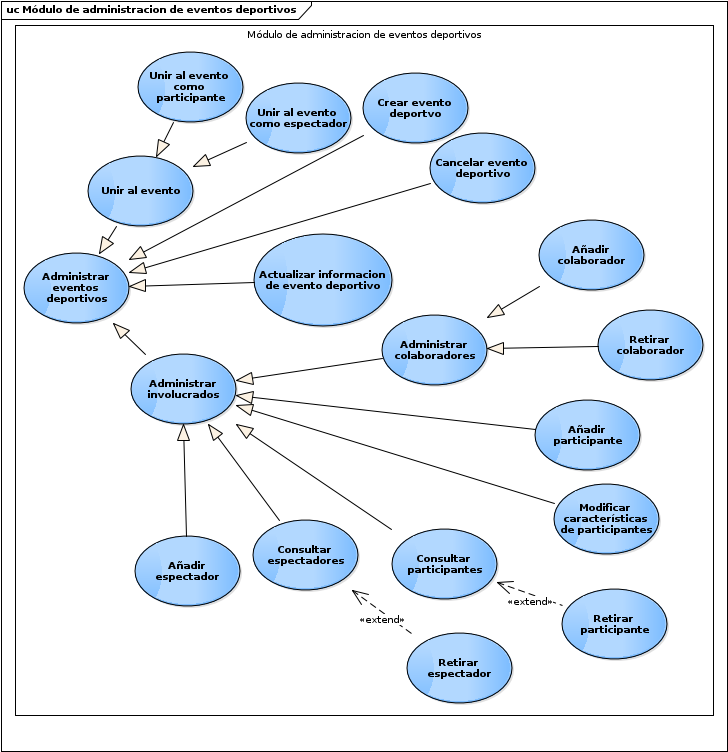
\includegraphics[width=11cm]{./imagenes/casos_uso/gestion_evento.png}
    \caption{Módulo de administración de eventos deportivos}
    \label{fig:cu_admin_eve}
    \textbf{Fuente:} Autores \\
  \end{center}
\end{figure}

En cuanto a éste módulo se refiere, los autores plasmaron las funcionalidades que se le ofrecen en el SNS a los organizadores de eventos deportivos, habiendo dos grandes módulos, a saber: Administración de involucrados y la gestión de la información del evento en si.

En el presente prototipo, los autores sólo implementarán la funcionalidad de creación de practicas deportivas debido a que es éso lo que se ha incluido en el alcance del proyecto.

\section{Módulo de gestión de administracion de deportes}

\begin{figure}[!htb]
  \begin{center}
    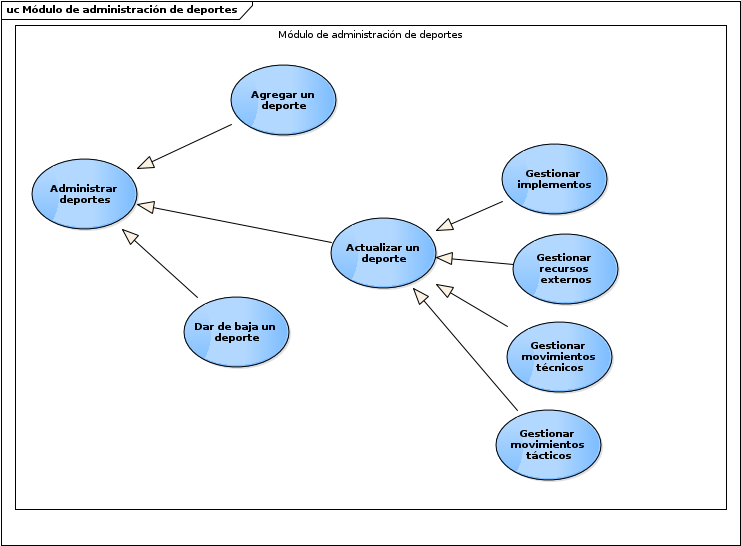
\includegraphics[width=11cm]{./imagenes/casos_uso/administracion_deportes.png}
    \caption{Módulo de gestión de administracion de deportes}
    \label{fig:cu_admin_dep}
    \textbf{Fuente:} Autores \\
  \end{center}
\end{figure}

Este módulo ofrece funcionalidades a los actores del sistema (especialmente el administrador) para administrar los deportes que éste juega, permitiendo al jugador dar información adicional de él en cada uno de los deportes que éste juega.

\section{Módulo de gestión de usuarios}

\begin{figure}[!htb]
  \begin{center}
    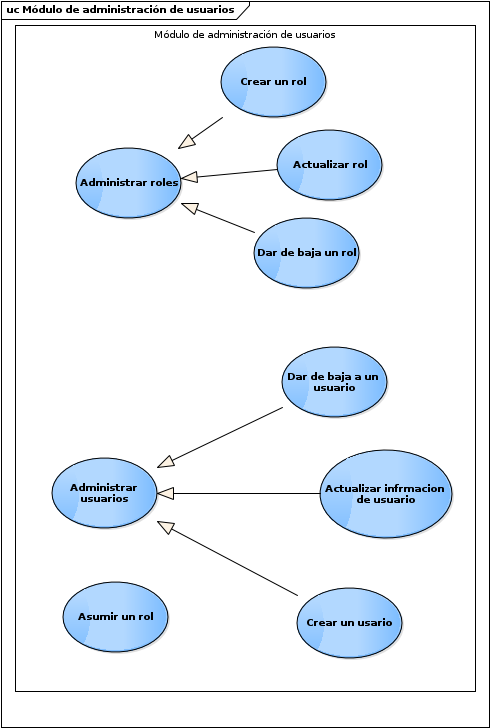
\includegraphics[width=11cm]{./imagenes/casos_uso/gestion_usuarios.png}
    \caption{Módulo de gestión de usuarios}
    \label{fig:cu_usuarios}
    \textbf{Fuente:} Autores \\
  \end{center}
\end{figure}

Este módulo ofrece a los usuarios la funcionalidad de administrar y gestionar su información como usuario de la aplicación (datos personales, datos de contacto)

\section{Módulo de gestión de ubicaciones}

\begin{figure}[!htb]
  \begin{center}
    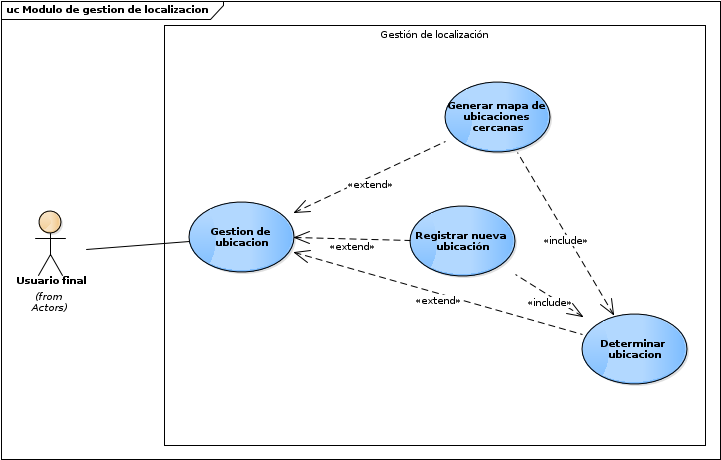
\includegraphics[width=11cm]{./imagenes/casos_uso/gestion_localizacion.png}
    \caption{Módulo de gestión de ubicaciones}
    \label{fig:cu_localizacion}
    \textbf{Fuente:} Autores \\
  \end{center}
\end{figure}

Este módulo ofrece a los usuarios la funcionalidad de obtener y utilizar su ubicación actual en la aplicación. El usuario puede utilizar esta información para obtener locaciones cercanas o registrar nuevas en la aplicación. Tambíen podrá utilizar su ubicación como insumo para los módulos de administración de torneos, administración de eventos deportivos, self-expression, difusión de información y gestión de patrocinios.